\chapter{Výsledková část}
Následující kapitola shrnuje získané výsledky pomocí CFD simulace popsané v předcházejících odstavcích. 

Na obr. \ref{fig:vecfield} je znázorněno vektorové pole rychlosti kapaliny v řezu nádobou a čase \SI{6}{\second}, což již lze považovat za poměrně ustálený stav. Z obrázku je dobře patrný vznikl sekundárních cirkulačních smyček v prostoru pod míchadlem. Tento jev byl experimentálně pozorován řadou autorů (např. \citet{hos10}) při zvolené světlé výšce míchadla od $C=T/2$ do $C=T/6$.  

\begin{figure}[h!]
\begin{center}
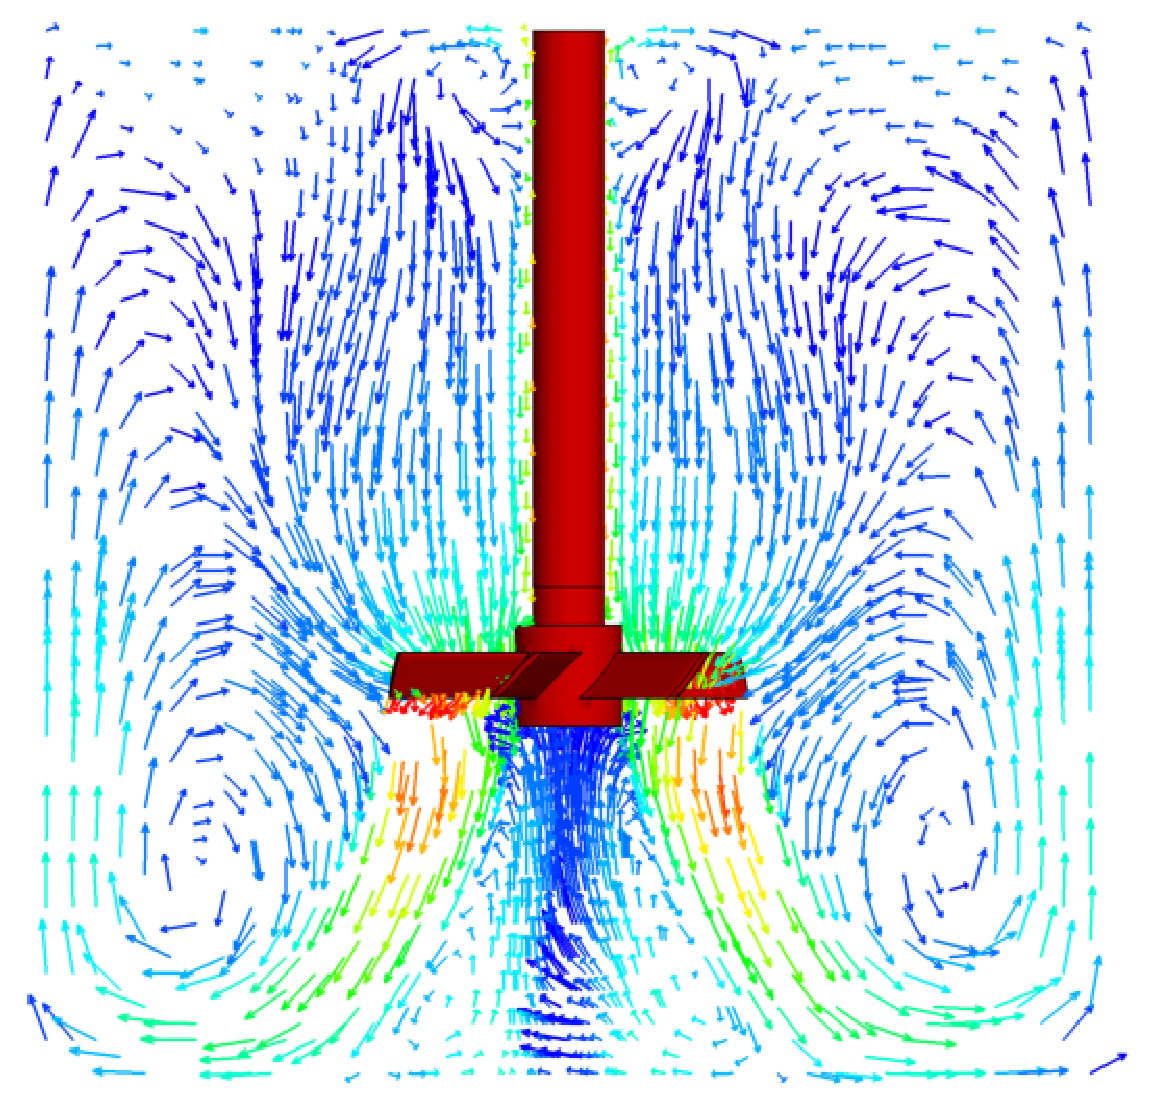
\includegraphics[scale=0.5]{images/vecfield.eps}
\caption{Vektorové pole rychlosti}
\label{fig:vecfield}
\end{center}
\end{figure} 

\vspace{-9mm}

Obr. \ref{fig:count2} zobrazuje kontury objemového zlomku pevné fáze v řezu míchací nádobou pro vybrané korelace odporového koeficientu. Tyto údaje byly získány v času simulace \SI{2}{\second}. Z obrázků je dobře patrné, že přímo pod míchadlem je největší koncentrace pevné fáze vlivem sekundárních cirkulačních smyček. Korelace odporového koeficientu podle Brucata v tomto případě předpovídá významně vyšší rozložení kuliček z PVC pod míchadlem než zbývající modely.

\newpage

\begin{figure}[h!]
  \begin{center}
  \subfloat[Schiller-Naumann]{\label{fig:neu2}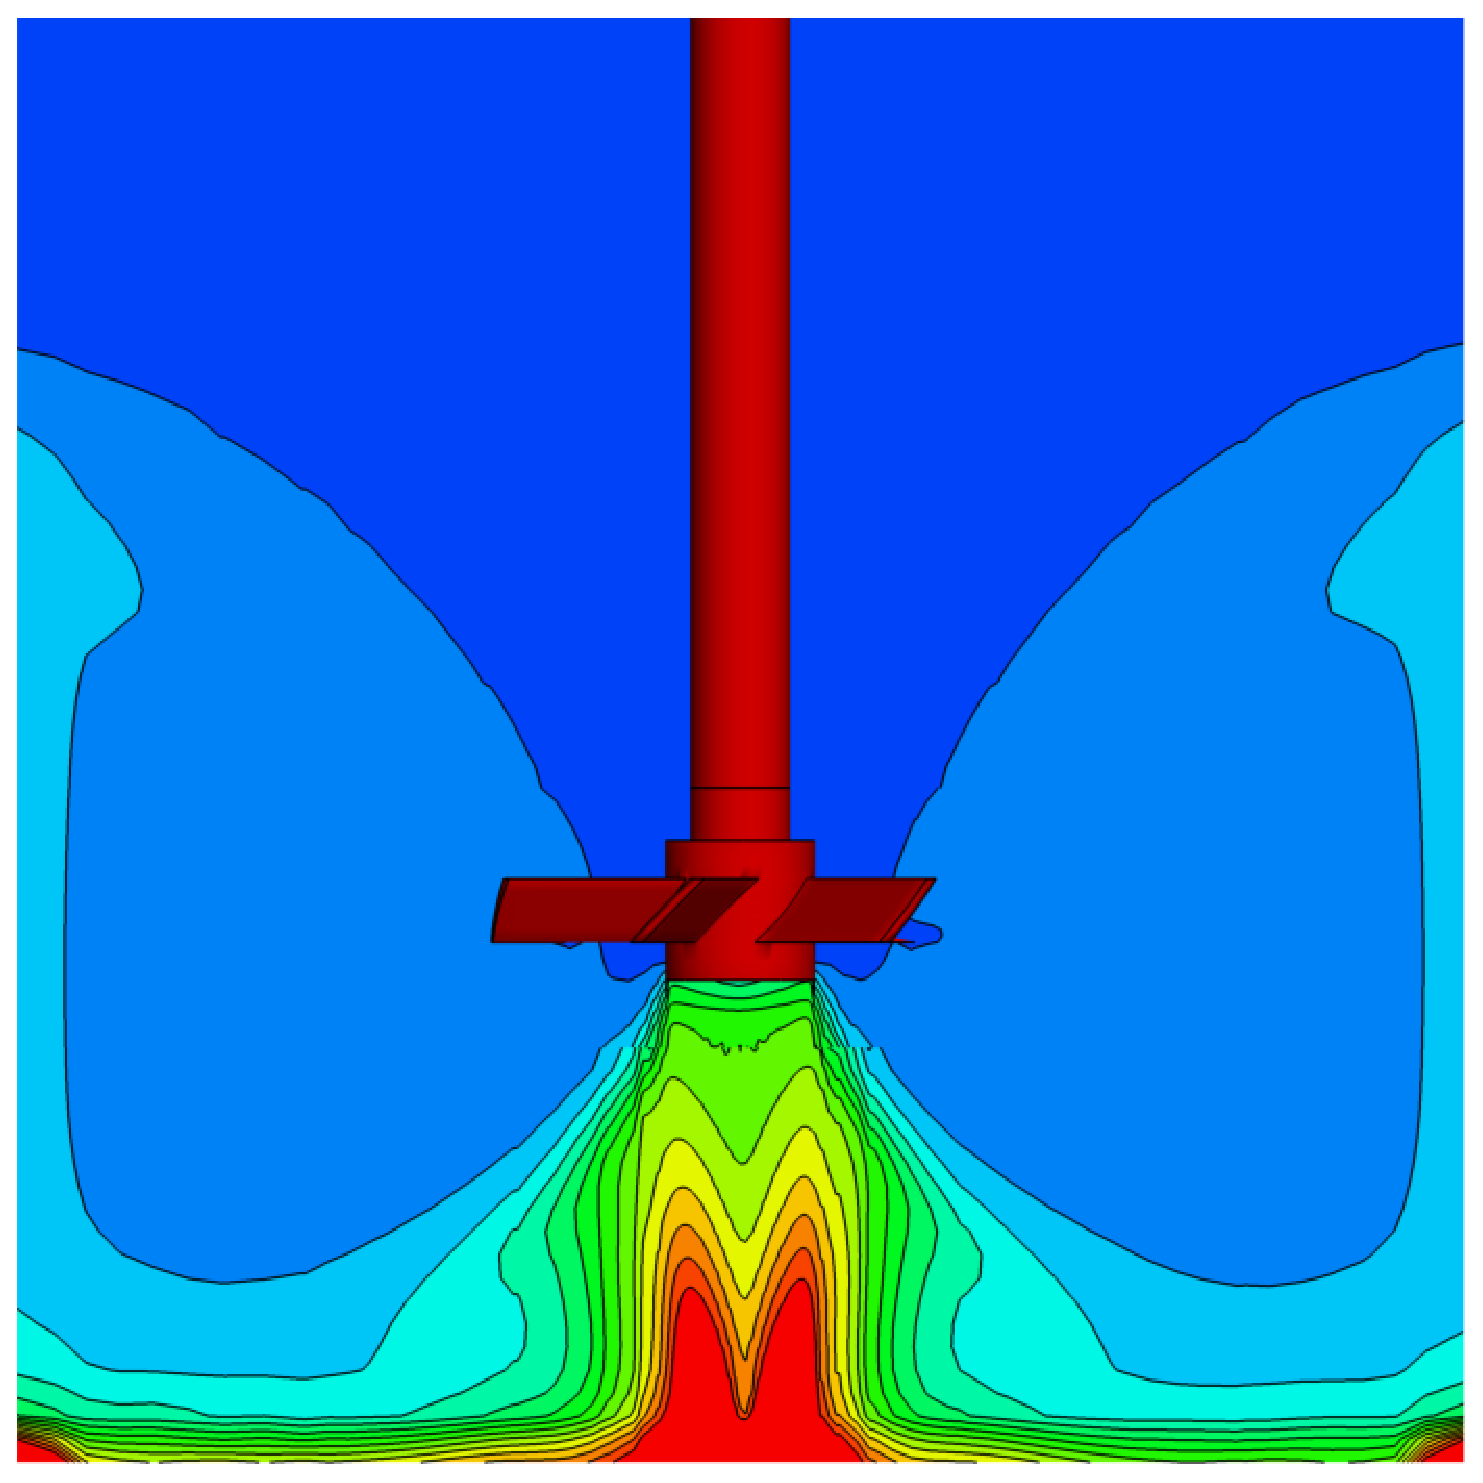
\includegraphics[scale=0.3]{images/volSch-2.eps}}  
  \qquad             
  \subfloat[Pinelli]{\label{fig:pin2}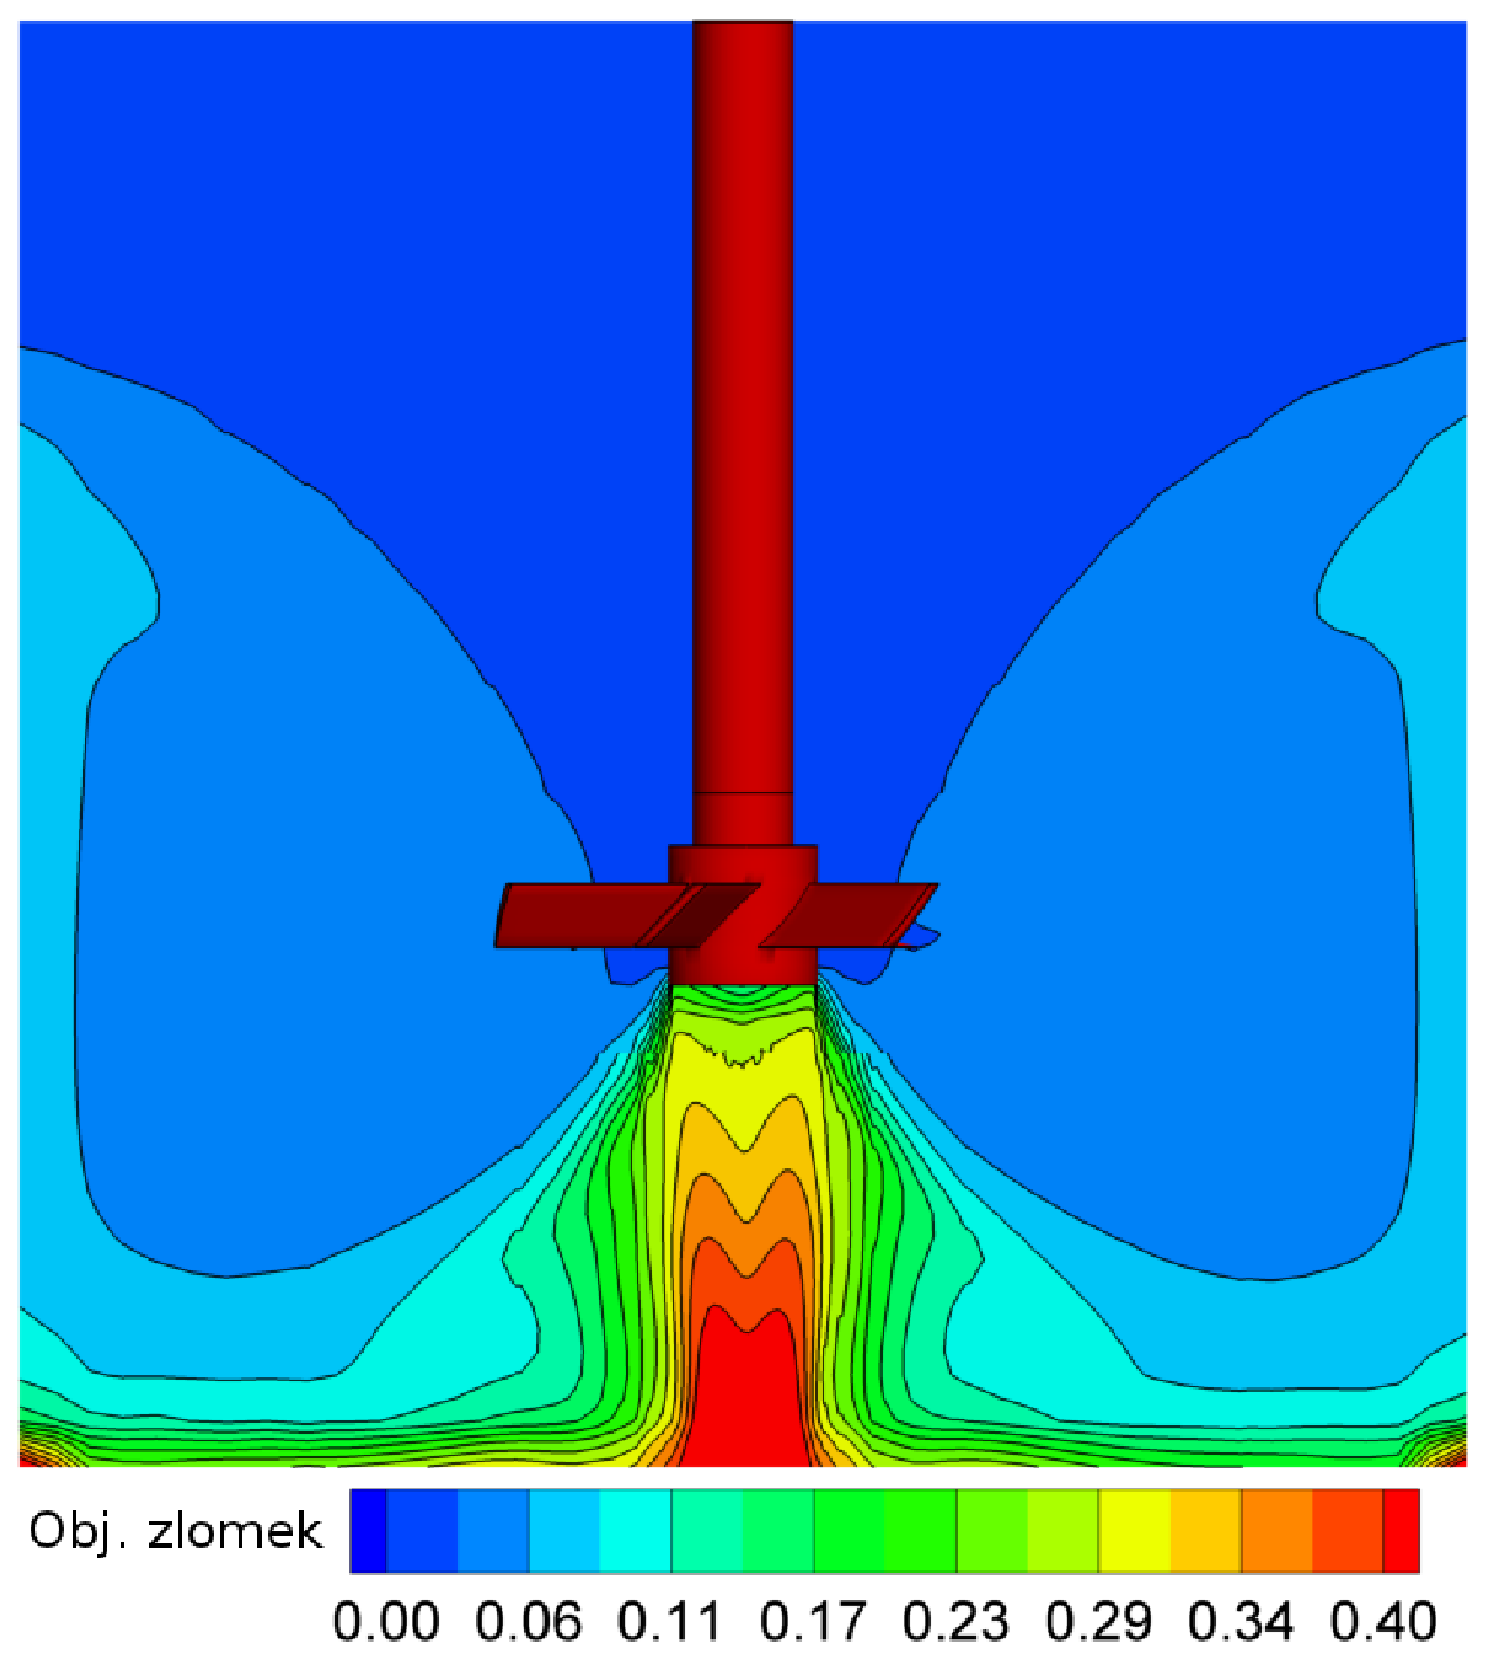
\includegraphics[scale=0.3]{images/volPin-2.eps}}
  \\
  \subfloat[Brucato]{\label{fig:bru2}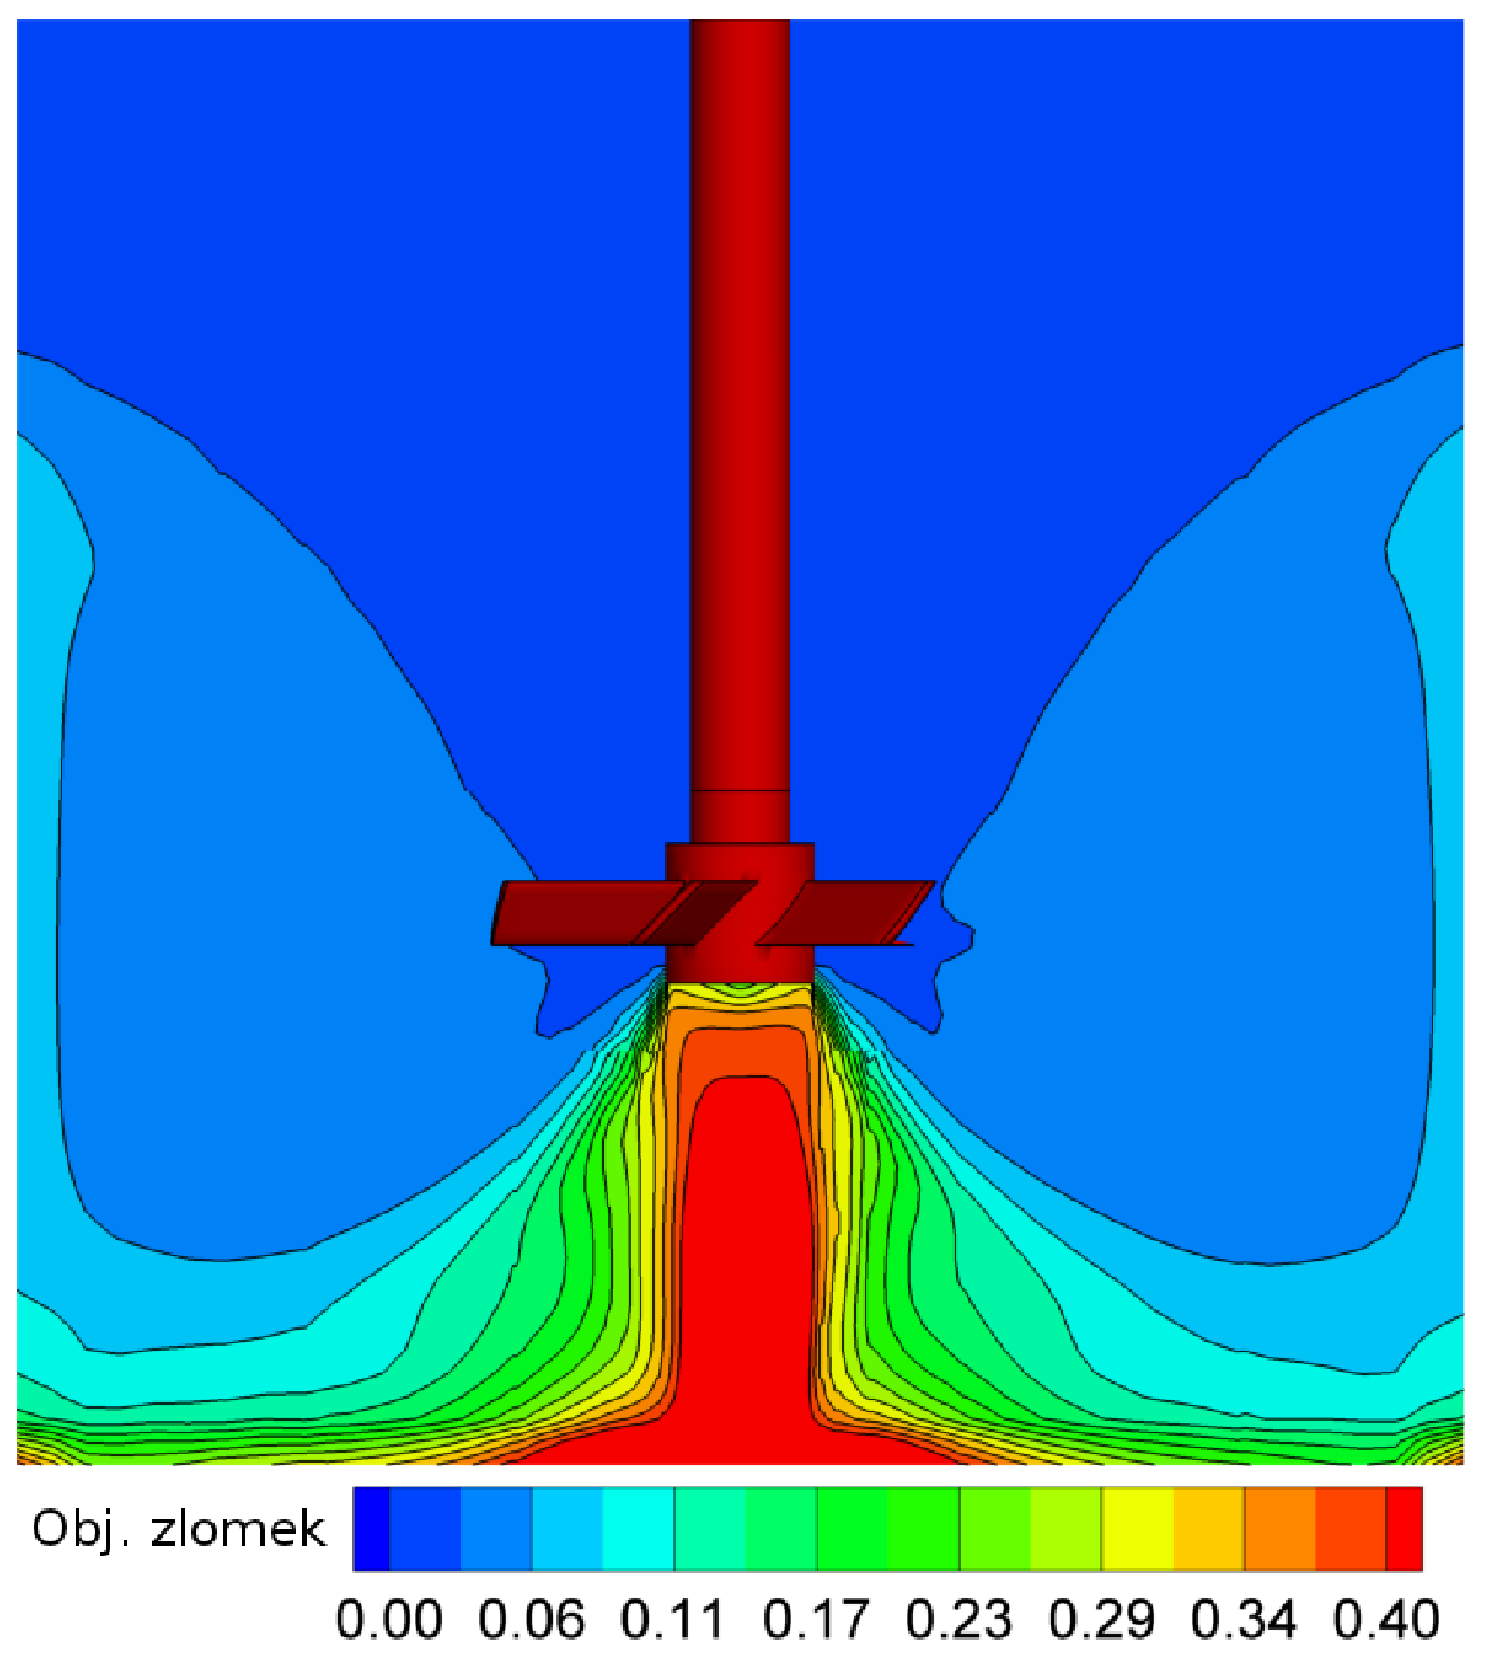
\includegraphics[scale=0.3]{images/volBru-2.eps}}
  \qquad
  \subfloat[Khopkar]{\label{fig:kho2}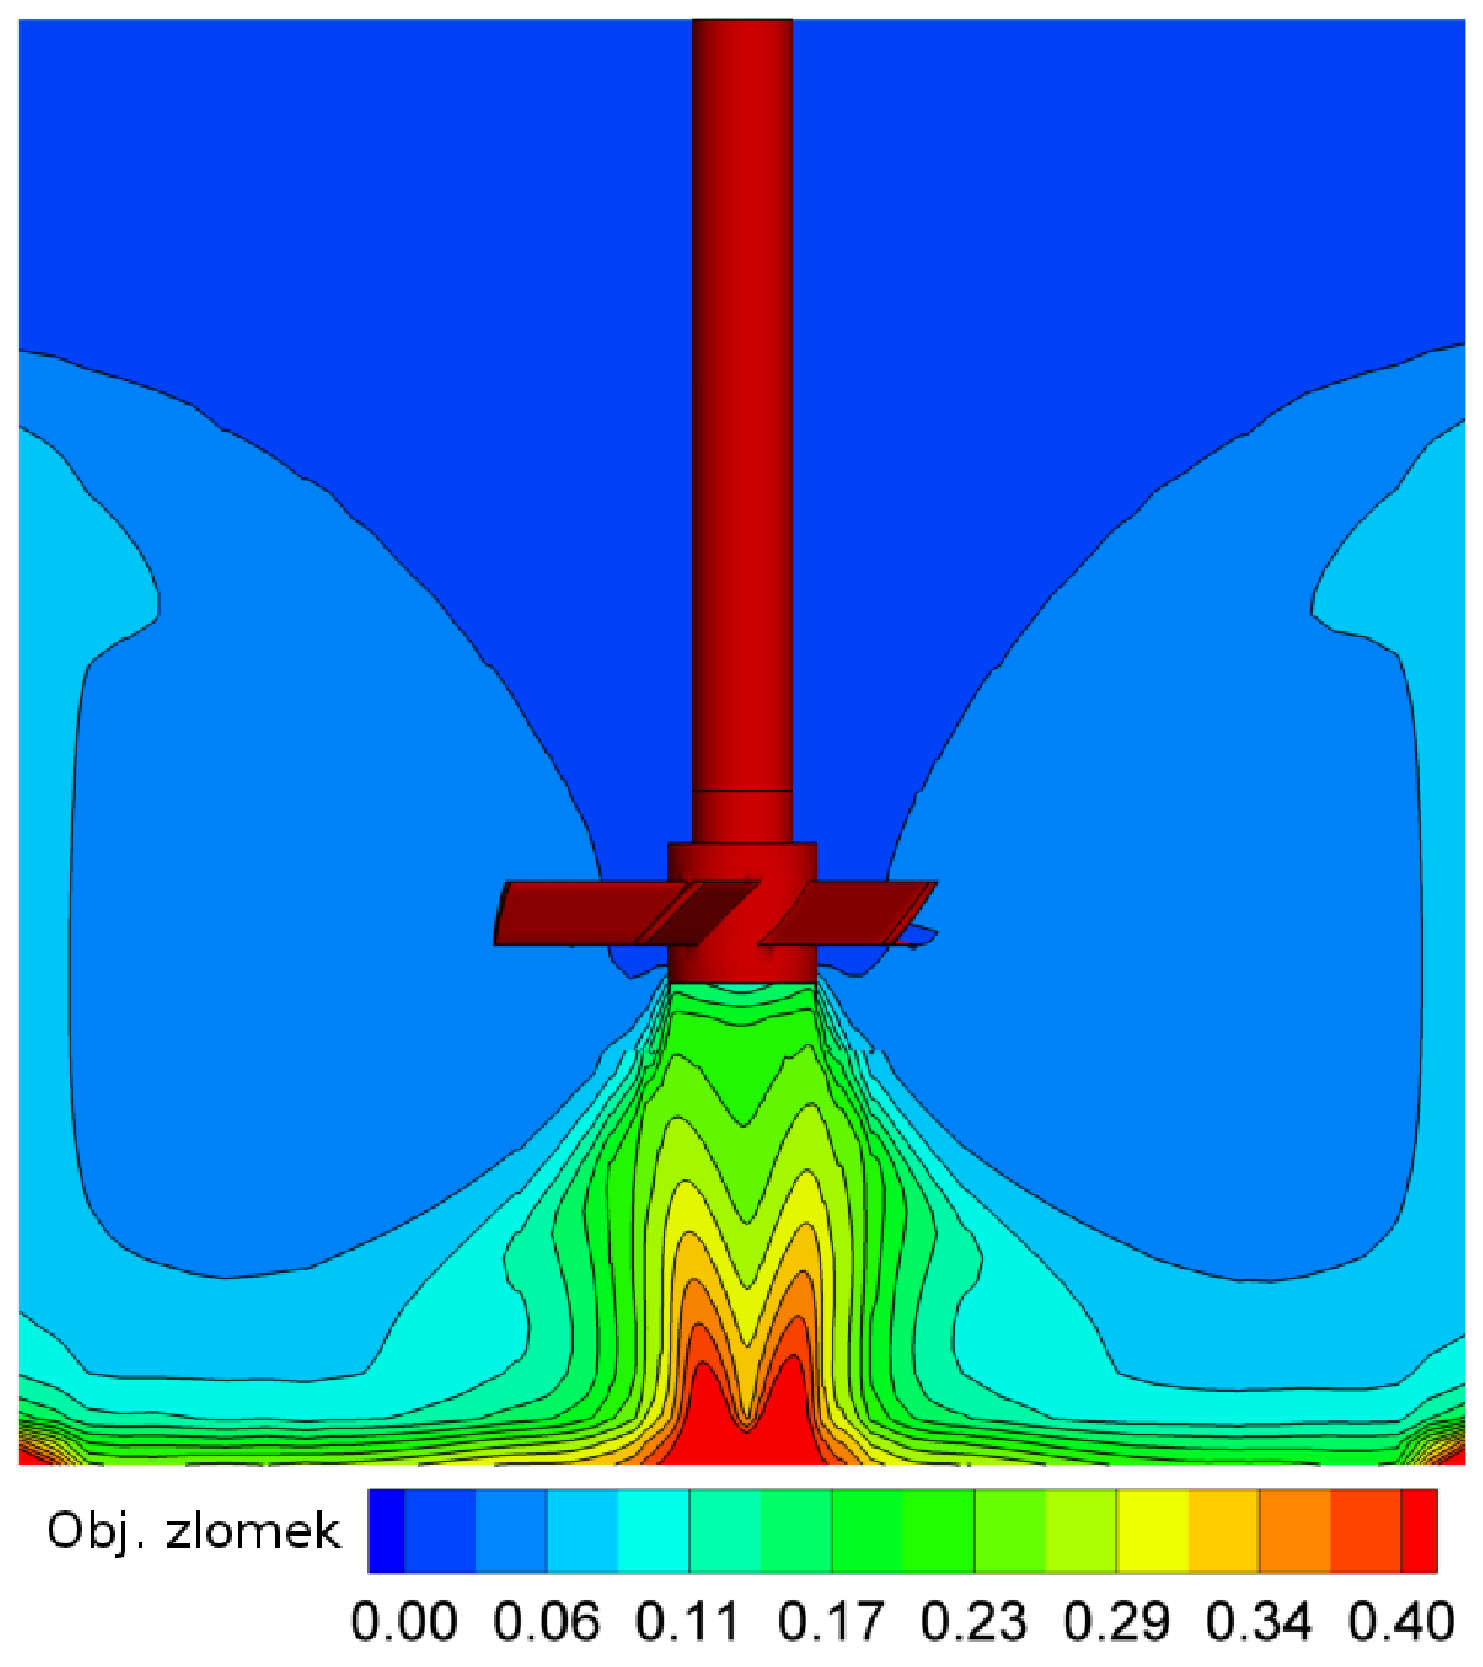
\includegraphics[scale=0.3]{images/volKho-2.eps}}
  \caption{Kocentrace pevné fáze v čase \SI{2}{\second}}
  \label{fig:count2}
  \end{center}
\end{figure}

\vspace{-9mm}

Následují opět obrázky zachycují objemový zlomek pevné fáze v řezu nádobou, avšak v tomto případě pro čas \SI{6}{\second}. Pevná fáze je již poměrně rozptýlena, ale stále se pod míchadlem nacházejí oblasti se zvýšenými koncentracemi.

\newpage

\begin{figure}[h!]
  \begin{center}
  \subfloat[Schiller-Naumann]{\label{fig:neu6}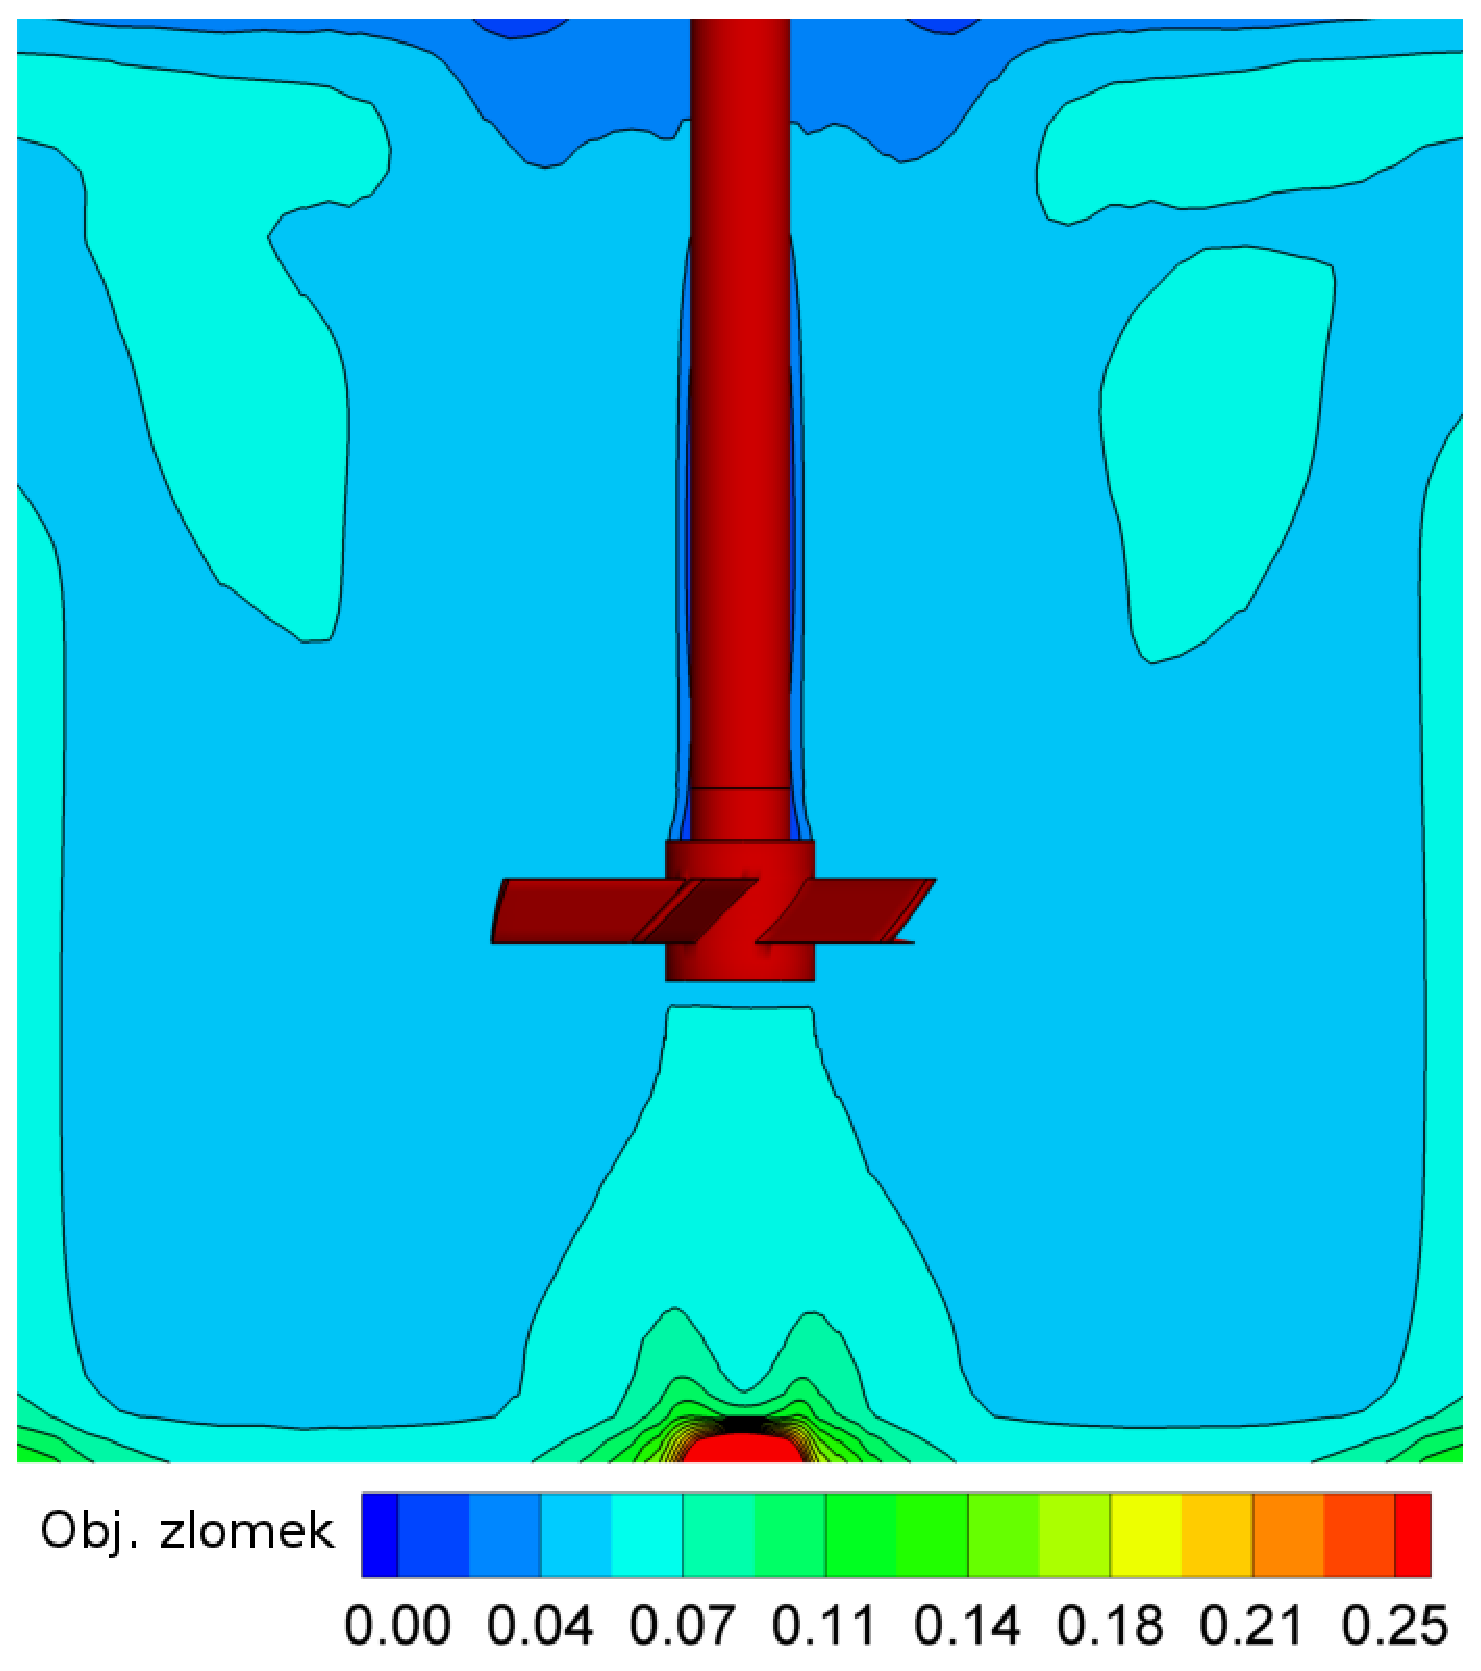
\includegraphics[scale=0.3]{images/volSch-6.eps}}  
  \qquad             
  \subfloat[Pinelli]{\label{fig:pin6}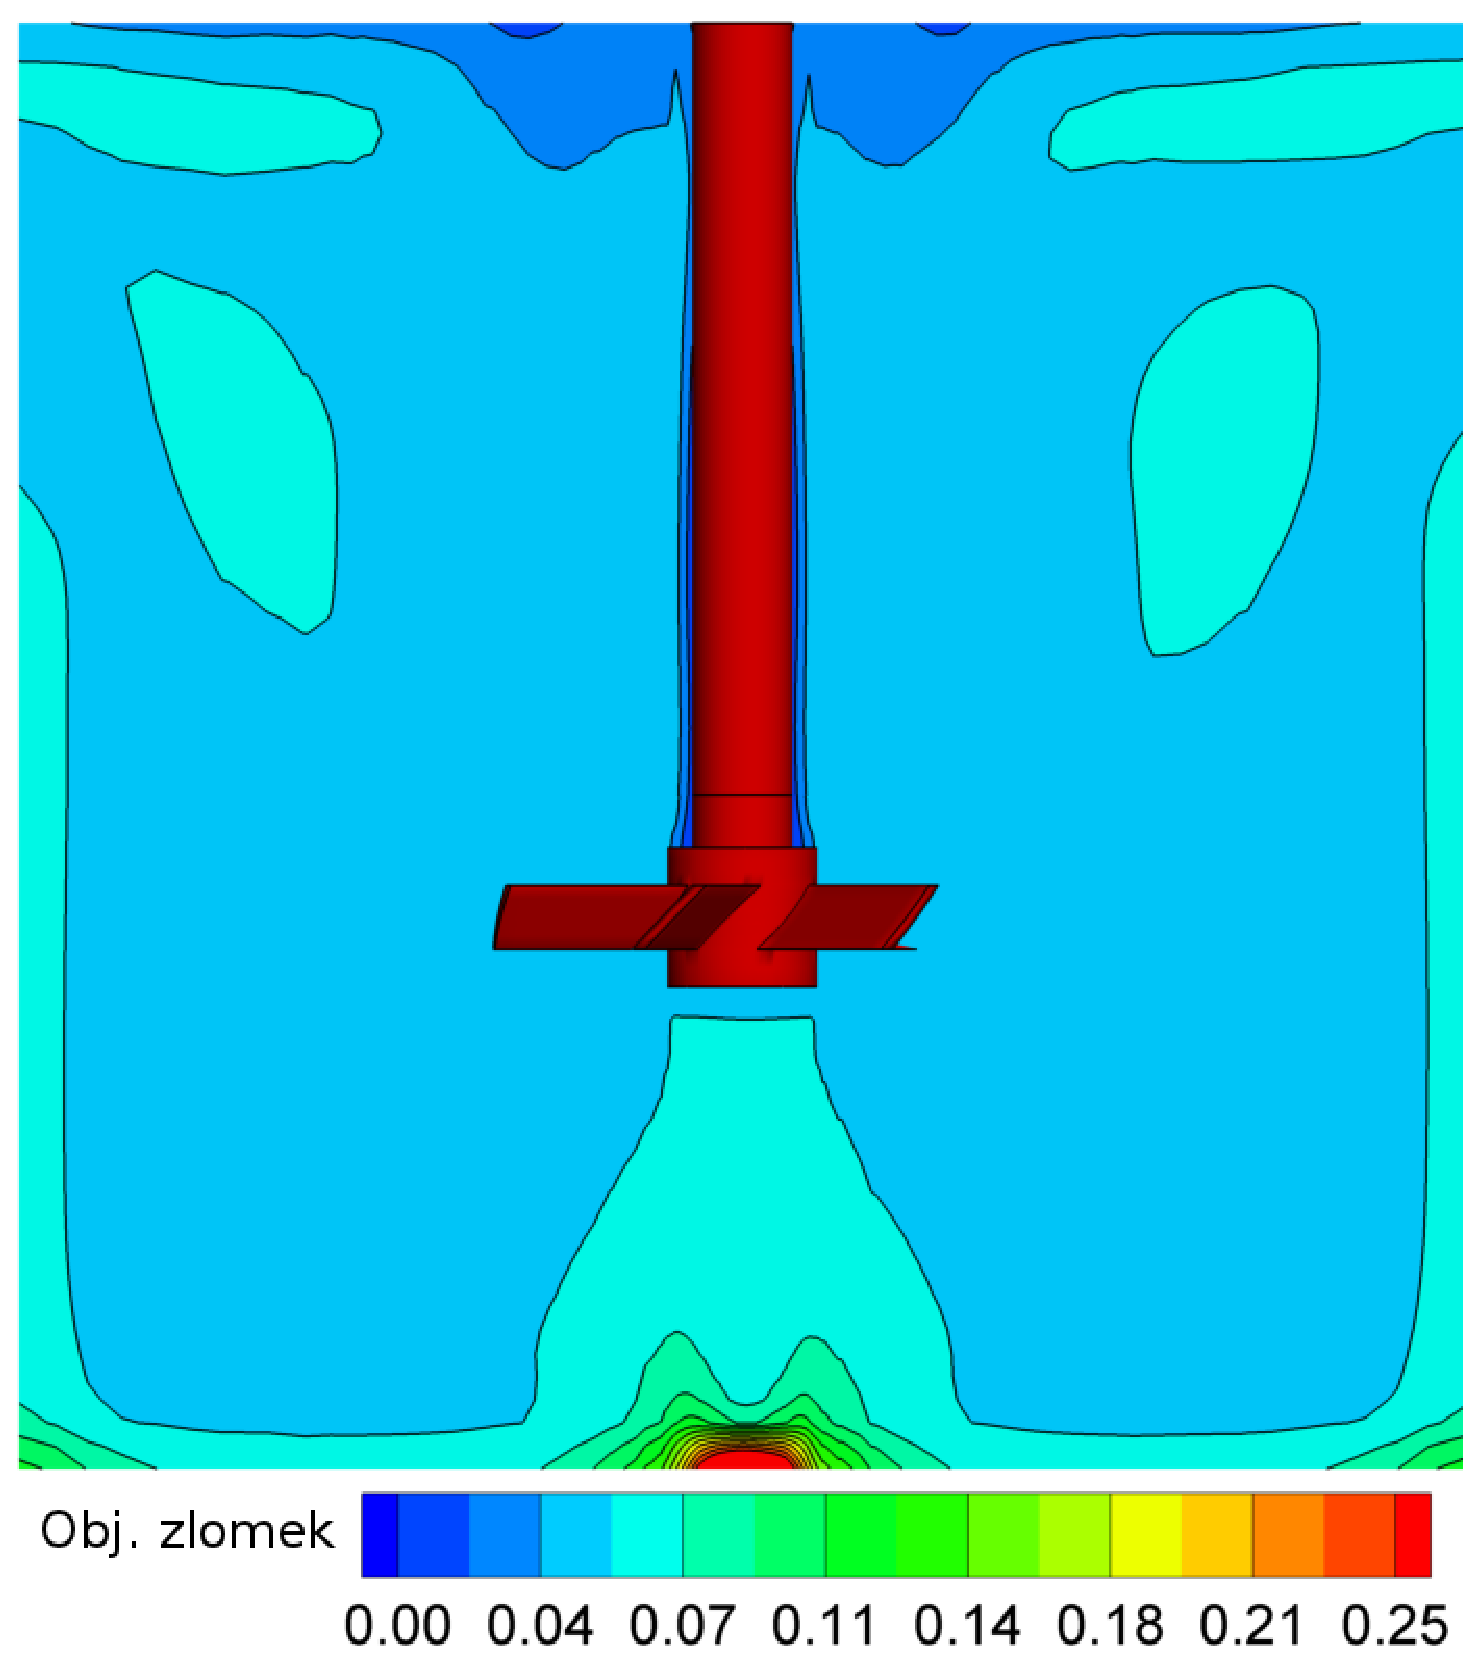
\includegraphics[scale=0.3]{images/volPin-6.eps}}
  \\
  \subfloat[Brucato]{\label{fig:bru6}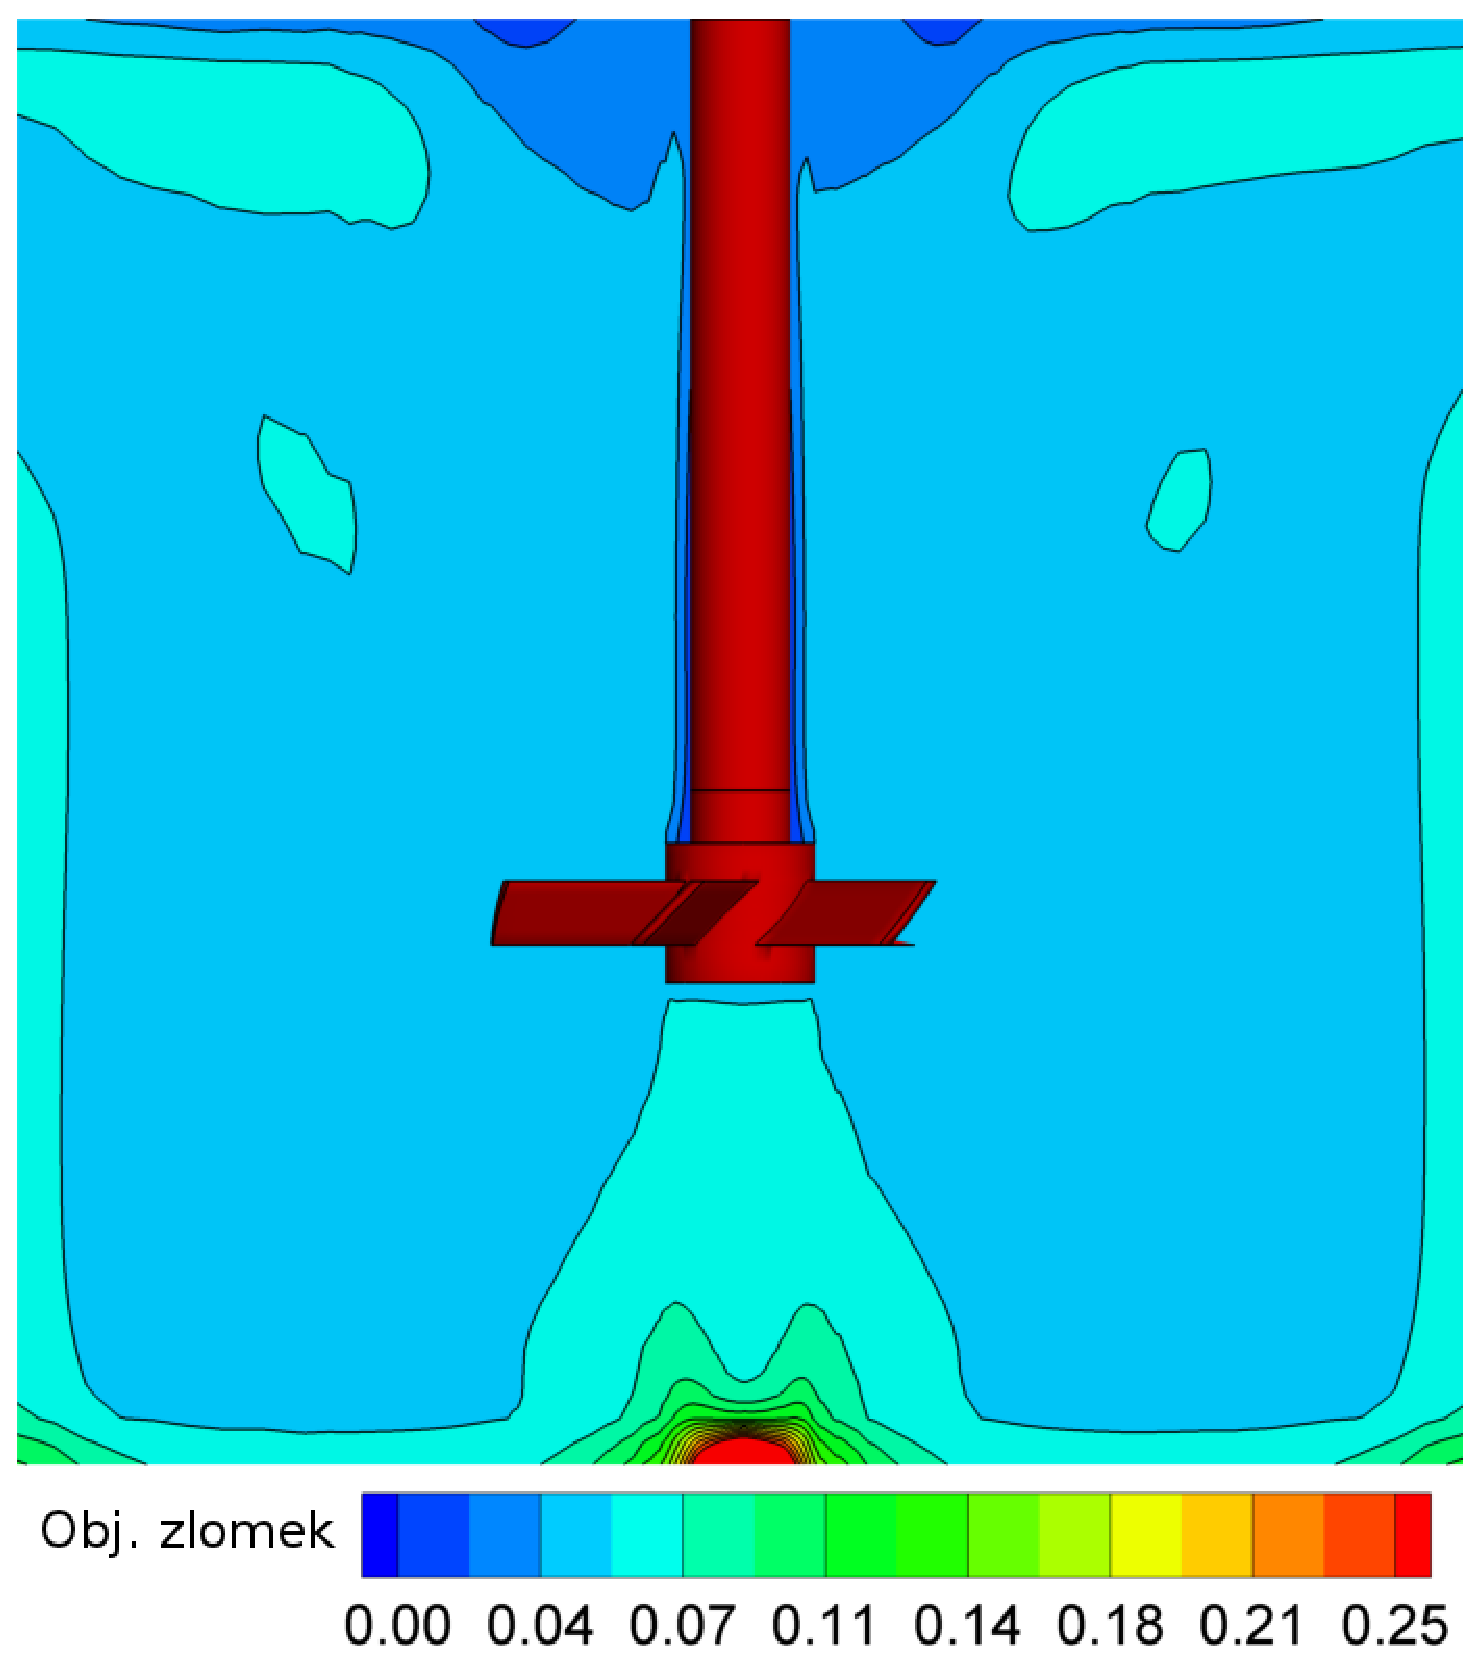
\includegraphics[scale=0.3]{images/volBru-6.eps}}
  \qquad
  \subfloat[Khopkar]{\label{fig:kho6}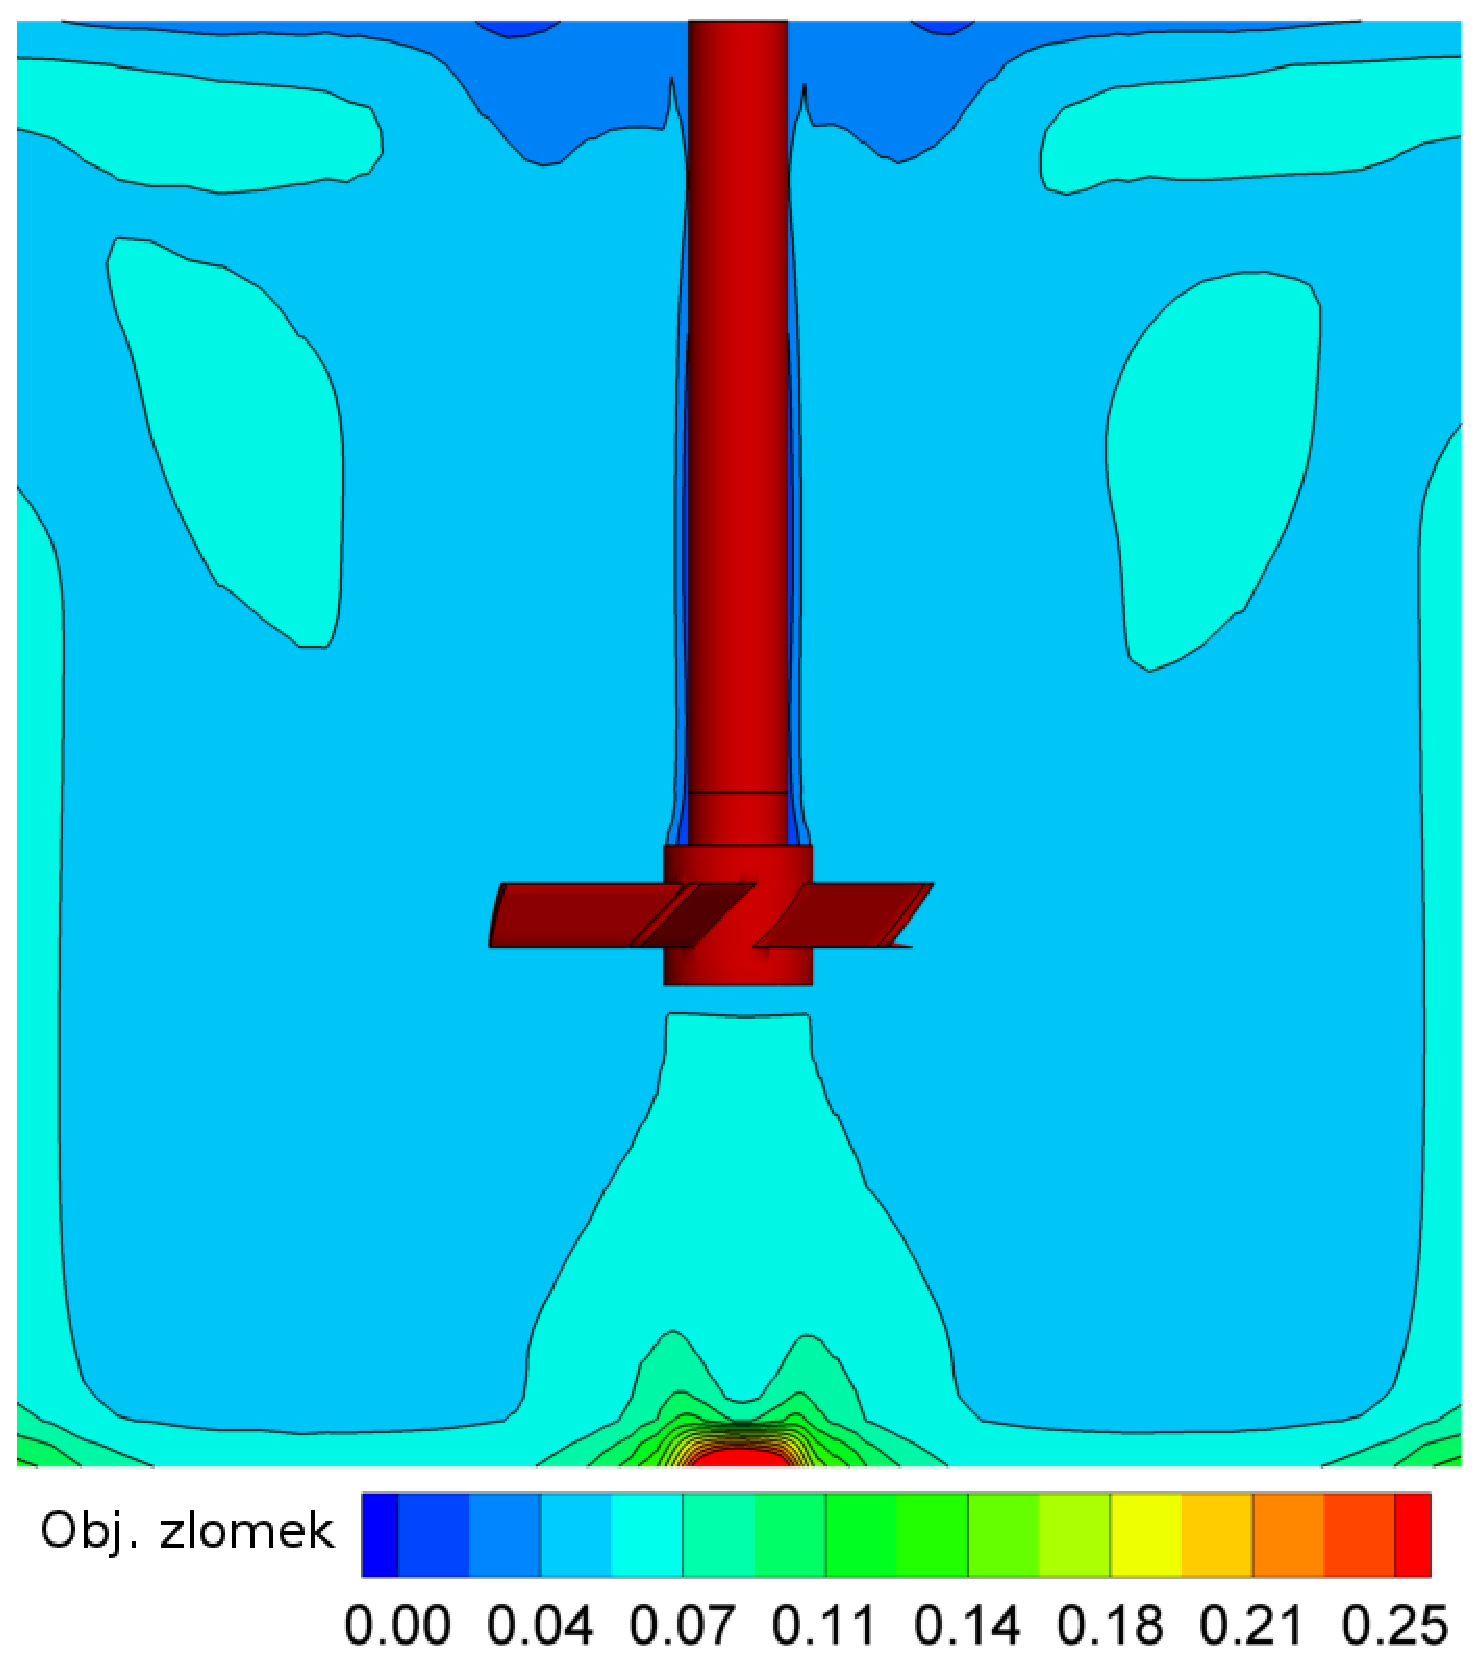
\includegraphics[scale=0.3]{images/volKho-6.eps}}
  \caption{Kocentrace pevné fáze v čase \SI{6}{\second}}
  \label{fig:count6}
  \end{center}
\end{figure}

\vspace{-9mm}

Následují grafické závislosti odporového koeficientu 

\newpage

\begin{figure}[h!]
\begin{center}
\includegraphics[scale=0.47]{images/Vol-2.eps}
\caption{Vektorové pole rychlosti}
\label{fig:vol2}
\end{center}
\end{figure} 

\vspace{-12mm}

\begin{figure}[h!]
\begin{center}
\includegraphics[scale=0.47]{images/Vol-6.eps}
\caption{Vektorové pole rychlosti}
\label{fig:vol6}
\end{center}
\end{figure} 

\vspace{-9mm}

Následují grafické závislosti odporového koeficientu 

\newpage

\begin{figure}[h!]
\begin{center}
\includegraphics[scale=0.47]{images/CD-2.eps}
\caption{Vektorové pole rychlosti}
\label{fig:cd2}
\end{center}
\end{figure} 

\vspace{-12mm}

\begin{figure}[h!]
\begin{center}
\includegraphics[scale=0.47]{images/CD-6.eps}
\caption{Vektorové pole rychlosti}
\label{fig:cd6}
\end{center}
\end{figure} 

\vspace{-9mm}

Následují grafické závislosti odporového koeficientu 

